\documentclass[12pt, a4paper, oneside]{ctexart}
\usepackage{amsmath, amsthm, amssymb, bm, color, graphicx, geometry, mathrsfs,extarrows, braket, booktabs, array}
\usepackage[colorlinks,linkcolor=red,anchorcolor=blue,citecolor=blue,urlcolor=blue,menucolor=black]{hyperref}
\setmainfont{Times New Roman}  % 设置英文字体
\setsansfont{Calibri}
\setmonofont{Consolas}

\linespread{1.4}
%\geometry{left=2.54cm,right=2.54cm,top=3.18cm,bottom=3.18cm}
\geometry{left=1.84cm,right=1.84cm,top=2.18cm,bottom=2.18cm}
\newenvironment{problem}{\par\noindent\textbf{题目. }}{\bigskip\par}
\newenvironment{solution}{\par\noindent\textbf{解答. }}{\bigskip\par}
\newenvironment{note}{\par\noindent\textbf{注记. }}{\bigskip\par}

%%%% 图片相对路径 %%%%
\graphicspath{{figure/}} % 当前目录下的figure文件夹, {../figure/}则是父目录的figure文件夹

\everymath{\displaystyle} % 默认全部行间公式
\DeclareMathOperator*\uplim{\overline{lim}} % 定义上极限 \uplim_{}
\DeclareMathOperator*\lowlim{\underline{lim}} % 定义下极限 \lowlim_{}
\let\leq=\leqslant % 将全部leq变为leqslant
\let\geq=\geqslant % geq同理

% 一些宏定义
\def\bd{\boldsymbol}        % 加粗(向量) boldsymbol
\def\disp{\displaystyle}    % 使用行间公式 displaystyle(默认)
\def\tsty{\textstyle}       % 使用行内公式 textstyle
\def\sign{\text{sign}}      % sign function
\def\wtd{\widetilde}        % 宽波浪线 widetilde
\def\R{\mathbb{R}}          % Real number
\def\N{\mathbb{N}}          % Natural number
\def\Z{\mathbb{Z}}          % Integer number
\def\C{\mathbb{C}}          % Complex number
\def\d{\mathrm{d}}          % differential operator
\def\e{\mathrm{e}}          % Euler's number
\def\i{\mathrm{i}}          % imaginary number
\def\re{\mathrm{Re}}        % Real part
\def\im{\mathrm{Im}}        % Imaginary part
\def\res{\mathrm{Res}}      % Residue
\def\L{\mathcal{L}}         % Loss function
\def\wdh{\widehat}          % 宽帽子 widehat
\def\ol{\overline}          % 上横线 overline
\def\ul{\underline}         % 下横线 underline
\def\add{\vspace{1ex}}      % 增加行间距
\def\del{\vspace{-3.5ex}}   % 减少行间距

% 基本信息
\newcommand{\RQ}{\today} % 日期
\newcommand{\km}{实变函数} % 科目
\newcommand{\bj}{强基数学002} % 班级
\newcommand{\xm}{吴天阳} % 姓名
\newcommand{\xh}{2204210460} % 学号

\begin{document}
% 正文部分

\section*{基础定义}
\textbf{集合}: 具有某种特性性质的具体的或抽象的对象的全体.

\textbf{元素}: 集合中的每一个对象.

\textbf{函数}: 设$X$为非空集, 若$f$将$X$中元素$x$对应到实数(复数), 则$f$为$X$上的实(复)函数.

\textbf{特征函数}: 设$X$为非空集, $A$为$X$的子集, 称
\begin{equation*}
    \chi_A=\begin{cases}
        1,&\quad x\in A,\\
        0,&\quad x\notin A,
    \end{cases}
\end{equation*}
为集$A$的特征函数.

\textbf{上极限与下极限}: $\uplim_{n\to\infty}A_n = \bigcap_{n=1}^\infty\bigcup_{m=n}^\infty A_m\quad \lowlim_{n\to\infty}A_n=\bigcup_{n=1}^\infty\bigcap_{m=n}^\infty A_m$.

\textbf{单调集列}: 设$\{A_n\}$为集列, 若$\forall n\in \N$, $A_n\subset A_{n+1}(A_{n+1}\subset A_n)$, 则称$\{A_n\}$为单增集列(单减集列), 统称为单调集列.

\textbf{映射(映照)}: 设$A, B$为非空集, 存在一个规则$\varphi$使得$\forall x\in A$, 按照规则$\varphi$都有一个确定的元素$y\in B$与$x$对应, 记为$\varphi:x\mapsto y$, 称$\varphi$是$A$到$B$的映射. $y$为$x$在$\varphi$下的像, 记$y = \varphi(x)$, $\varphi^{-1}(y) = \{x\in A: \varphi(x) = y\}$. 定义域为$A = \mathcal{D}_\varphi$, 值域$\varphi(A) = \mathcal{R}_\varphi$.

\textbf{映射的延拓}: $\varphi,\psi$为$\mathcal{D}_\varphi, \mathcal{D}_\phi$到$B$的映射, 若$\mathcal{D}_\varphi\subset \mathcal{D}_\psi$且$\forall x\in \mathcal{D}_\varphi$有$\psi(x)=\varphi(x)$, 则$\psi$为$\varphi$在$\mathcal{D}_\psi$上的延拓, 记$\varphi\subset\psi$, 称$\varphi$为$\psi$在$\mathcal{D}_\varphi$上的限制, 记为$\varphi = \psi|_{\mathcal{D}_\varphi}$.

\textbf{复合映射}: $\varphi_1:A\to B$, $\varphi_2:B\to C$, 作$\varphi:A\to C$, 使得$\forall x\in A$, 有$\varphi(x) = \varphi_2(\varphi_1(x))$, 称$\varphi$为$\varphi_1,\varphi_2$的复合映射, 记为$\varphi_2\circ\varphi_1$.

\textbf{单射(可逆映射)}: $\varphi:A\to B$, $\forall y\in \mathcal{R}_\varphi$, 存在唯一的$x\in A$使得$\varphi(x) = y$, 称$\varphi$为单射.

\textbf{双射(一一对应)}: $\varphi$为集合$A$到集合$B$上的单射, 即$\mathcal{R}(\varphi) = B$, 则称$\varphi$为双射.

\textbf{逆映射}: 令$\varphi:A=\mathcal{D}_\varphi\to\mathcal{R}_\varphi\subset B$, 若$\varphi:x\mapsto y$, $x\in A, y\in B$, 则令$\psi:y\mapsto x$, 称$\psi$为$\varphi$的逆映射, 记$\psi$为$\varphi^{-1}$.

\textbf{恒等映射}: 设$A$为集合, 称$A$到$A$的映射$\varphi:x\mapsto x$为$A$上的恒等映射.

\textbf{对等}: 设$A,B$为两个集, 若存在$A$到$B$的双射$\varphi$, 则称集$A$与集$B$对等(相似), 记$A\sim B$.

\textbf{势}: 设$A$为非空集, 所有与$A$对等的集合所构成的类, 称为$A$的势或者基数, 记为$\ol{\ol{A}},|A|, \text{Card}(A)$.

\textbf{有限集}: 设$A$为非空集, 若存在$n\in\N$, 使得$A\sim\{1, 2,\cdots, n\}$, 则称$A$是有限集.

\textbf{无限集}: 设$A$为非空集, 若$A$不是有限集, 则称$A$为无限集.

\textbf{可数集}: 设$A$为非空集, 若$A\sim \N$, 则称$A$为可数集.

\textbf{至多可数集}: 设$A$为非空集, 若$A$为有限集或可数集, 则称$A$为至多可数集.

\textbf{不可数集}: 设$A$为非空集, 若$A$不是至多可数集, 则称$A$为不可数集.

\textbf{可数集}: 设$A$为非空集, 

\textbf{关系}: 设$X, Y$为两个集合, 若$R$为$X\times Y$的一个子集, 即$R\subset X\times Y$, 则称$R$为$X$到$Y$的一个关系. 特别的, $X$到其自身上的关系称为$X$上的关系.

\textbf{相关的}: 设$R$为$X$到$Y$的一个关系, 若$(x, y)\in R$, 则称$x$与$y$是$R$-相关的, 记做$xRy$.

\textbf{剖分}: 设$X$为一个集, $\{X_i,i\in I\}$是$X$的一族子集, 若满足 (1) $X_i\cap X_j = \varnothing, (i\neq j)$; (2) $\bigcap_{i\in I}X_i = X$, 则称$\{X_i,i\in I\}$为$X$的一个剖分.

\textbf{构成区间}: 设$G$为直线上的开集, 若开区间$(a, b)\subset G$, 且端点$a, b$不属于$G$, 则称$(a, b)$为$G$的一个构成区间.

\textbf{开集, 极限点, 孤立点, 导集, 闭集, 闭包}

\textbf{自密集}: $A\subset A'$.

\textbf{完全集}: $A'=A$.

\textbf{稠密集}: $A, B\subset \R$, 若$\forall b\in B$, $\exists \varepsilon > 0$, 使得$(b-\varepsilon, b+\varepsilon)\cap A\neq \varnothing$, 则$A$在$B$中稠密, 当$B=\R$时, $A$为稠密集.

\textbf{疏朗集}: $S\subset \R$, 若$S$在任意的开区间中都不稠密, 则$S$为疏朗集(也称无处稠密集).

\textbf{集类(类), 基本空间}: $E\in 2^X$, 则$E$为$X$上的集类, $X$为$E$的基本空间.

\textbf{环}: $R$为$X$上的非空集类, 若$\forall E_1, E_2\in R$有$E_1\cup E_2\in R$, $E_1-E_2\in R$, 则$R$为$X$上的环, 若$X\in R$, 则称$R$为$X$上的代数.

\textbf{$\sigma$环}: 设$S$为$X$上的集类, 任意一列$E_i\in S$均有$\bigcup_{i=1}^\infty E_i\in S,\ E_1-E_2\in S$, 则称$S$为$X$上的$\sigma$环, 若$X\in S$, 则$S$为$X$上的$\sigma$域.

\textbf{单调类}: $M$为$X$上的集类, 若对$M$中任意单调集列$\{E_n\}$有$\lim_{n\to\infty}E_n\in M$, 则$M$为单调类.

\textbf{集函数}: 设$\R_* = \R\cup\{\infty, -\infty\}$, 若$\mu:E\to\R_*$, 其中$E$为集类, 则$\mu$为集函数.

\textbf{环$R$上的测度}: $R$为$X$上的环, $\mu$为$R$上的集函数, 若$\mu$满足:

(1) $\mu(\varphi) = 0$; (2) $\forall E\in R$, $\mu(E)\geq 0$;

(3) 任何一列两两不交的集列$E_i\in R$, 且$\bigcup_{i=1}^\infty E_i\in R$, 则$\mu\left(\bigcup_{i=1}^\infty\right) = \sum_{i=1}^\infty\mu(E_i)$.

\textbf{$\mu$零集}: 设$\mu:R\to \R$为集函数, 若$E\in R$使得$\mu(E) = 0$, 则称$E$为$\mu$零集.

\textbf{完备测度}: $\mu$零集的子集都属于$R$, 则$\mu$为$R$上的完备测度.

\textbf{外侧度}: $R$为$X$上的环, $\mu$为$R$上的测度, 令$\mu^*:H(R)\to\R$, 定义为
\begin{equation*}
    \mu^*(E) = \inf\left\{\sum_{k=1}^\infty \mu(E_k):\{E_k\}\subset R, E\subset \bigcup_{k=1}^\infty E_k\right\}
\end{equation*}
其中$H(R) = \{E\subset X: \text{存在}R\text{中的集列覆盖}E\}$, 称$\mu^*$为$\mu$诱导的外侧度.

\textbf{Caratheodory条件}: $\mu^*$为$R$上测度$\mu$所诱导的外侧度, $E\in H(R)$, 若$E$满足$\forall F\in H(R)$有 
\begin{equation*}
\mu^*(F) = \mu^*(E\cap F) +\mu^*(F-E),
\end{equation*}
则称$E$为$\mu^*$可测集, 全体 $\mu^*$可测集构成的集类记为$R^*$.

\textbf{有限测度}: $R$为$X$上的环, $\mu$为$R$上的测度

(1) $\forall E\in R$, $\mu(E) < \infty$, 称$\mu$为有限测度.

(2) $\forall E\in R$, 存在$\{E_i\}\subset R$, 使得$E\subset \bigcup_{i=1}^\infty E_i$且$\forall i\in \N$, $\mu(E_i) < \infty$, 则称$\mu$为$\sigma$有限测度.

(3) 代数上的有限测度称为全有限测度, 代数上的$\sigma$有限测度称为全$\sigma$有限测度.

\textbf{Lebesgue测度}: $\R^n$上半开半闭有限长方体全体所成的半环$P$, 设$m:P\to \R$, 为
\begin{equation*}
    m\left(\prod_{i=1}^m(a_i, b_i]\right) = \prod_{i=1}^n(b_i-a_i),
\end{equation*}
$\tilde{m}$为环$R_0 = R(P)$上的测度, 记$\tilde{m}$为$m$, 称$\sigma$环$R_0^*$上的测度$m^*$为Lebesgue测度. $R_0^*$为Lebesgue可测集, 称$\mathcal{L} = R_0^*$为Lebesgue可测集类.

\def\B{\mathcal{B}}

\textbf{Borel类}: $\B = R_{\sigma}(R_0)$.

\textbf{等测包}: $E\subset \R$, 存在$H\in \L$, 且$E\subset H$, 且$m^*(E) = m^*(H)$, 则称$H$为$E$的等测包.

\textbf{可测空间}: 设$R$为$X$上的$\sigma$环, 且$X=\bigcup_{E\in R}E$, 则称$(X, R)$为可测空间, $R$中元素称为$(X, R)$中的可测集.

\textbf{Lebesgue可测空间}: $(\R^n, \L)$为Lebesgue可测空间, $\L$中元素为Lebesgue可测集.

\textbf{Borel可测空间}: $(\R^n, \B)$为Borel可测空间, $\B$中元素为Borel可测集.

\textbf{可测函数}: 设$(X, R)$为可测空间, $E\subset X$, $f:E\to\R$, 若$\forall t\in \R$, 由$\{x\in E:f(x)\geq t\}\in R$, 则称$f$为$E$上关于$(X, R)$的可测函数.

\textbf{简单函数}: 设$(X, R)$为可测空间, $E\in R$, 若$f:E\to \R$可表示为$f(x) = \sum_{i=1}^k\alpha_i\chi_{E_i}(x)$, 其中$\varphi_1,\cdots, \varphi_k\in \R,\ E_1,\cdots, E_k\in R$两两不交, 且$\bigcup_{i=1}^kE_i\subset E$, 则称$f$为$E$上的简单函数.

\textbf{测度空间}: 设$(X, R)$为可测空间, $\mu$为$R$上的测度, 则$(X, R,\mu)$为测度空间. 当$\mu$为$R$上的有限测度, 全有限测度, $\sigma$有限测度, 全$\sigma$有限测度时, 称$(X, R, \mu)$分别为有限测度空间, 全有限测度空间, $\sigma$有限测度空间, 全$\sigma$有限测度空间(在后面加上空间就行了).

\textbf{Lebesgue测度空间}: 称$(\R, \L, m)$为Lebesgue测度空间.

\textbf{几乎处处}: 设$(X, R, \mu)$为测度空间, $E\subset X$, P为一个关于$E$的命题, 若$\exists E_0\subset X$使得$\mu(E_0) = 0$, 且$\forall x\in E-E_0$, 命题P成立, 则称命题P在$E$撒花姑娘几乎处处成立, 记$P(x)\ a.e.\ in\ E$.

\textbf{几乎处处有限, 相等, 收敛}: $f,g,f_k:E\to\R_*$, $\exists E_0\subset X$使得$\mu(E_0) = 0$且$|f(x)| < \infty,\  f(x) = g(x),\ \lim_{k\to\infty}f_k(x) = f(x)\ (x\in E-E_0)$.

\textbf{几乎可测}: $f:E\to\R_*$, 存在$h:E\to\R_*$及$E_0\subset X$使得$\mu(E_0) = 0$, 且$f(x) = h(x),\ (x\in E-E_0)$.

\textbf{依测度收敛}: 设$(X, R, \mu)$为测度空间, $E\subset X$, $\{f_n\}$为$E$上的可测函数, $f:E\to\R$为$E$上的有限函数, 若$\forall \varepsilon > 0$, 有$\lim_{n\to\infty}\mu(E(|f_k-f| > \varepsilon)) = 0$, 则称$\{f_k\}$为$E$上依测度$\mu$收敛于$f$.

\textbf{依测度基本列}: 设$(X, R, \mu)$为测度空间, $E\subset X$, $\{f_k\}$为$E$上可测函数列, 若$\forall \varepsilon,\delta>0$, $\exists K\in \N$, 使得
\begin{equation*}
    \mu(E(|f_k-f_j| > \varepsilon)) < \delta \quad (k, j > K)
\end{equation*}
则称$\{f_k\}$为依测度基本列.

\textbf{近一致收敛}: 设$(X, R, \mu$为测度空间, $E\in R$, $f, f_1, f_2,\cdots$为$E$上广义实值函数, 若$\forall \delta > 0$, $\exists E_\delta \subset E$使得$\mu(E-E_\delta) < \delta$且在$E_\delta$上, $\{f_k\}$一致收敛于$f$, 则$\{f_k\}$在$E$上近一致收敛于$f$.

\textbf{非负简单函数积分}: 设$(X, R, \mu$为测度空间, $E\in R$, 设$f$为$X$上的非负简单函数, $f=\sum_{i=1}^pc_i\chi_{A_i}$, 其中$c_1,\cdots, c_p\geq 0$, $A_1,\cdots, A_p\in R$两两不交, 称
\begin{equation*}
    \int_Ef\,\d \mu:=\sum_{i=1}^pc_i\mu(E\cap A_i)
\end{equation*}
为$f$在$E$上的积分.

\textbf{非负可测函数的积分}: 设$(X, R, \mu$为测度空间, $E\in R$, $f$为$E$上的非负广义实值可测函数, 记$H_f = \{h:h\text{为}X\text{上的非负简单函数且}f|_E\leq f\}$, 称
\begin{equation*}
    \int_Ef\,\d \mu:=\sum\left\{\int_Eh\,\d \mu:h\in H_f\right\}
\end{equation*}
为$f$在$E$上的积分, 若$\int_Ef\,\d \mu < \infty$, 则称$f$为$E$上的可积函数.

\textbf{正部, 负部}: 设$(X, R, \mu$为测度空间, $E\in R$, $f$为$E$上广义实值可测函数, 记
\begin{equation*}
    f^+=\max(f, 0),\qquad f^-=\min(f, 0),
\end{equation*}
称$f^+$为$f$的正部, $f^-$为$f$的负部.

\textbf{一般可测函数的积分}: 设$(X, R, \mu$为测度空间, $E\in R$, $f$为$E$上的广义实值可测函数, 若非负可测函数$f^+, f^-$的积分$\int_Ef^+\,\d \mu$和$\int_Ef^-\,\d \mu$中至少一个是有限值, 则称
\begin{equation*}
    \int_Ef\,\d \mu = \int_Ef^+\,\d \mu - \int_Ef^-\,\d \mu
\end{equation*}
为$f$在$E$上的积分, 若$f^+$和$f^-$都为$E$上的可积函数, 则$f$为$E$上的可积函数, 称$f$在$E$上可积.

% 下面给一些功能的写法
\iffalse
% 图片模板
\centerline{
    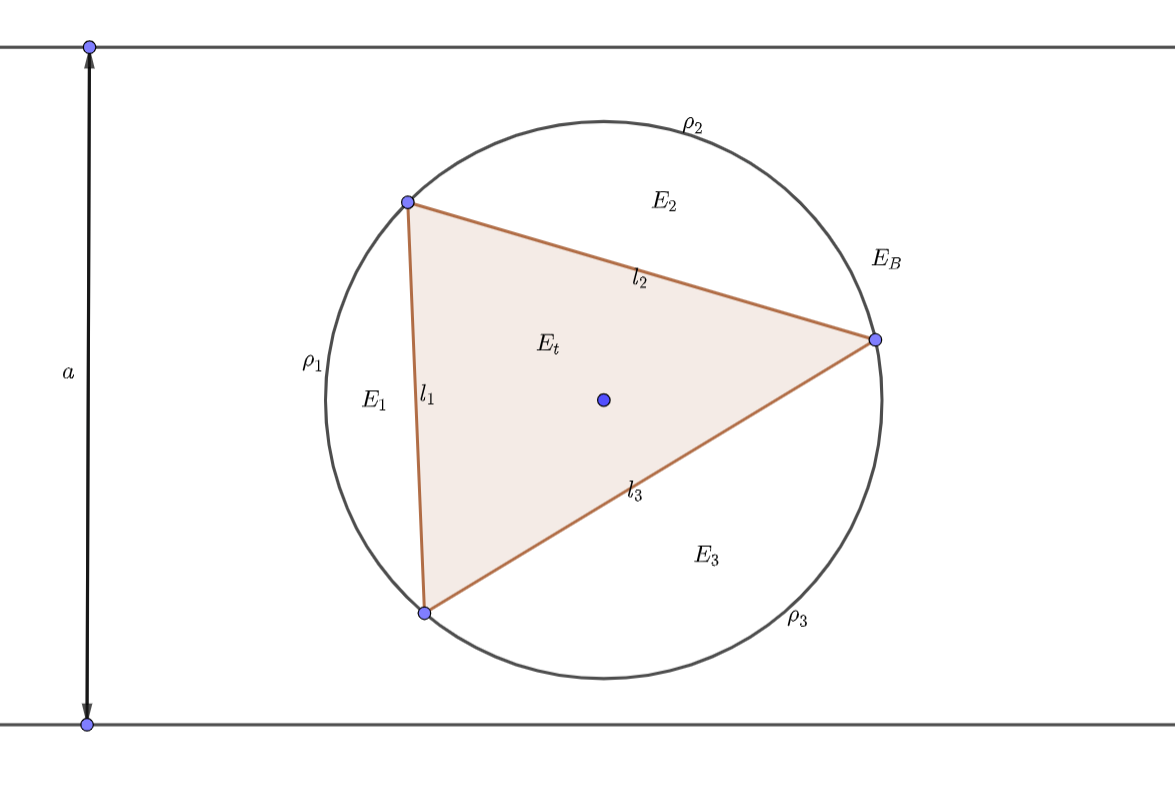
\includegraphics[width=0.8\textwidth]{figure.png}
}
% 表格模板
\renewcommand\arraystretch{0.8} % 设置表格高度为原来的0.8倍
\begin{table}[!htbp] % table标准
    \centering % 表格居中
    \begin{tabular}{p{1cm}<{\centering}p{1cm}<{\centering}p{3cm}<{\centering}p{5cm}<{\centering}} % 设置表格宽度
    %\begin{tabular}{cccc}
        \toprule
        $x_i$ & $f[x_1]$ & $f[x_i,x_{i+1}]$ & $f[x_i,x_{i+1},x_{i+2}]$ \\
        \midrule
        $x_0$ & $f(x_0)$ &                  &                          \\
        $x_0$ & $f(x_0)$ & $f'(x_0)$        &                          \\
        $x_0$ & $f(x_1)$ & $\frac{f(x_1)-f(x_0)}{x_1-x_0}$ & $\frac{f(x_1)-f(x_0)}{(x_1-x_0)^2}-\frac{f'(x_0)}{x_1-x_0}$\\
        \bottomrule
    \end{tabular}
\end{table}

\def\Log{\text{Log}} % 一个简单的宏定义
$\Log$ % 调用方法
\fi

\end{document}